\documentclass{beamer}

\usepackage[utf8]{inputenc}
\usepackage[T1]{fontenc}
\usepackage[english]{babel}
\usepackage{amsmath}
\usepackage{amsfonts}
\usepackage{amssymb}
\usepackage{amsthm}
\usepackage{mystmaryrd}
\usepackage{xspace}
\usepackage{mathpartir}
\usepackage{mymacros}
\usepackage{textcomp}
\usepackage{tikz}
\usepackage{pifont}

\def\ok{\ding{52}}
\def\bad{\ding{56}}
\definecolor{lgreen}{rgb}{0.8,1,0.8}
\definecolor{pink}{rgb}{1.0,0.8,0.8}

% EBNF syntax.

\let\nt\textit % Nonterminal.
\newcommand{\is}{& ${} ::= {}$ &}
\newcommand{\optional}[1]{$[\,\text{#1}\,]$} % Option.
\newcommand{\seplist}[2]{#2#1${}\ldots{}$#1#2}
\newcommand{\sepspacelist}[1]{\seplist{\ }{#1}}
\newcommand{\sepcommalist}[1]{\seplist{,\ }{#1}}
\newcommand{\newprod}{\\\hskip 1cm\barre\hskip2mm}
\newcommand{\phaprod}{\\\hskip 1cm\phantom\barre\hskip2mm}

% Concrete syntax.

\newcommand{\percentpercent}{\kw{\%\%}\xspace}
\newcommand{\deuxpoints}{\kw{:}\xspace}
\newcommand{\barre}{\kw{\textbar}\xspace}
\newcommand{\kangle}[1]{\kw{\textless} #1 \kw{\textgreater}}
\newcommand{\ocamltype}{\kangle{\textit{\ocaml type}}\xspace}
\newcommand{\ocamlparam}{\kangle{\nt{uid} \deuxpoints \textit{\ocaml module type}}\xspace}
\newcommand{\dheader}[1]{\kw{\%\{} #1 \kw{\%\}}}
\newcommand{\dtoken}{\kw{\%token}\xspace}
\newcommand{\dstart}{\kw{\%start}\xspace}
\newcommand{\dtype}{\kw{\%type}\xspace}
\newcommand{\dnonassoc}{\kw{\%nonassoc}\xspace}
\newcommand{\dleft}{\kw{\%left}\xspace}
\newcommand{\dright}{\kw{\%right}\xspace}
\newcommand{\dparameter}{\kw{\%parameter}\xspace}
\newcommand{\dpublic}{\kw{\%public}\xspace}
\newcommand{\dinline}{\kw{\%inline}\xspace}
\newcommand{\donerrorreduce}{\kw{\%on\_error\_reduce}\xspace}
\newcommand{\dpaction}[1]{\kw{\{} #1 \kw{\}}\xspace}
\newcommand{\daction}{\dpaction{\textit{\ocaml code}}\xspace}
\newcommand{\dprec}{\kw{\%prec}\xspace}
\newcommand{\dequal}{\kw{=}\xspace}
\newcommand{\dquestion}{\kw{?}\xspace}
\newcommand{\dplus}{\kw{+}\xspace}
\newcommand{\dstar}{\kw{*}\xspace}
\newcommand{\dlpar}{\kw{(}\,\xspace}
\newcommand{\drpar}{\,\kw{)}\xspace}
\newcommand{\eos}{\kw{\#}\xspace}
\newcommand{\dnewline}{\kw{\textbackslash n}\xspace}

% Stylistic conventions.

\newcommand{\kw}[1]{\text{\upshape\sf\bfseries #1}}
\newcommand{\inlinesidecomment}[1]{\textit{\textbf{\footnotesize // #1}}}
\newcommand{\sidecomment}[1]{\hskip 2cm\inlinesidecomment{#1}}
\newcommand{\docswitch}[1]{\vspace{1mm plus 1mm}#1.\hskip 3mm}
\newcommand{\error}{\kw{error}\xspace}

% Abbreviations.

\newcommand{\menhir}{Menhir\xspace}
\newcommand{\menhirlib}{\texttt{MenhirLib}\xspace}
\newcommand{\menhirlibconvert}{\href{http://gallium.inria.fr/~fpottier/menhir/convert.mli.html}{\texttt{MenhirLib.Convert}}\xspace}
\newcommand{\menhirinterpreter}{\texttt{MenhirInterpreter}\xspace}
\newcommand{\menhirlibincrementalengine}{\href{http://gallium.inria.fr/~fpottier/menhir/IncrementalEngine.ml.html}{\texttt{MenhirLib.IncrementalEngine}}\xspace}
\newcommand{\menhirlibgeneral}{\href{http://gallium.inria.fr/~fpottier/menhir/general.mli.html}{\texttt{MenhirLib.General}}\xspace}
\newcommand{\cmenhir}{\texttt{menhir}\xspace}
\newcommand{\ml}{\texttt{.ml}\xspace}
\newcommand{\mli}{\texttt{.mli}\xspace}
\newcommand{\mly}{\texttt{.mly}\xspace}
\newcommand{\ocaml}{OCaml\xspace}
\newcommand{\ocamlc}{\texttt{ocamlc}\xspace}
\newcommand{\ocamlopt}{\texttt{ocamlopt}\xspace}
\newcommand{\ocamldep}{\texttt{ocamldep}\xspace}
\newcommand{\ocamlfind}{\texttt{ocamlfind}\xspace}
\newcommand{\make}{\texttt{make}\xspace}
\newcommand{\omake}{\texttt{omake}\xspace}
\newcommand{\ocamlbuild}{\texttt{ocamlbuild}\xspace}
\newcommand{\Makefile}{\texttt{Makefile}\xspace}
\newcommand{\yacc}{\texttt{yacc}\xspace}
\newcommand{\bison}{\texttt{bison}\xspace}
\newcommand{\ocamlyacc}{\texttt{ocamlyacc}\xspace}
\newcommand{\ocamllex}{\texttt{ocamllex}\xspace}
\newcommand{\token}{\texttt{token}\xspace}
\newcommand{\automaton}{\texttt{.automaton}\xspace}
\newcommand{\conflicts}{\texttt{.conflicts}\xspace}
\newcommand{\dott}{\texttt{.dot}\xspace}

% Files in the distribution.

\newcommand{\distrib}[1]{\texttt{#1}}

% Environments.

\newcommand{\question}[1]{\vspace{3mm}$\diamond$ \textbf{#1}}

% Ocamlweb settings.

\newcommand{\basic}[1]{\textit{#1}}
\let\ocwkw\kw
\let\ocwbt\basic
\let\ocwupperid\basic
\let\ocwlowerid\basic
\let\ocwtv\basic
\newcommand{\ocwbar}{\vskip 2mm plus 2mm \hrule \vskip 2mm plus 2mm}
\newcommand{\tcup}{${}\cup{}$}
\newcommand{\tcap}{${}\cap{}$}
\newcommand{\tminus}{${}\setminus{}$}

% Command line options.

\newcommand{\obase}{\texttt{-{}-base}\xspace}
\newcommand{\ocomment}{\texttt{-{}-comment}\xspace}
\newcommand{\odepend}{\texttt{-{}-depend}\xspace}
\newcommand{\orawdepend}{\texttt{-{}-raw-depend}\xspace}
\newcommand{\odump}{\texttt{-{}-dump}\xspace}
\newcommand{\oerrorrecovery}{\texttt{-{}-error-recovery}\xspace}
\newcommand{\oexplain}{\texttt{-{}-explain}\xspace}
\newcommand{\oexternaltokens}{\texttt{-{}-external-tokens}\xspace}
\newcommand{\ofixedexc}{\texttt{-{}-fixed-exception}\xspace}
\newcommand{\ograph}{\texttt{-{}-graph}\xspace}
\newcommand{\oignoreone}{\texttt{-{}-unused-token}\xspace}
\newcommand{\oignoreall}{\texttt{-{}-unused-tokens}\xspace}
\newcommand{\oinfer}{\texttt{-{}-infer}\xspace}
\newcommand{\oinspection}{\texttt{-{}-inspection}\xspace}
\newcommand{\ointerpret}{\texttt{-{}-interpret}\xspace}
\newcommand{\ointerpretshowcst}{\texttt{-{}-interpret-show-cst}\xspace}
\newcommand{\ologautomaton}{\texttt{-{}-log-automaton}\xspace}
\newcommand{\ologcode}{\texttt{-{}-log-code}\xspace}
\newcommand{\ologgrammar}{\texttt{-{}-log-grammar}\xspace}
\newcommand{\onoinline}{\texttt{-{}-no-inline}\xspace}
\newcommand{\onostdlib}{\texttt{-{}-no-stdlib}\xspace}
\newcommand{\oocamlc}{\texttt{-{}-ocamlc}\xspace}
\newcommand{\oocamldep}{\texttt{-{}-ocamldep}\xspace}
\newcommand{\oonlypreprocess}{\texttt{-{}-only-preprocess}\xspace}
\newcommand{\oonlytokens}{\texttt{-{}-only-tokens}\xspace}
\newcommand{\ostrict}{\texttt{-{}-strict}\xspace}
\newcommand{\osuggestcomp}{\texttt{-{}-suggest-comp-flags}\xspace}
\newcommand{\osuggestlinkb}{\texttt{-{}-suggest-link-flags-byte}\xspace}
\newcommand{\osuggestlinko}{\texttt{-{}-suggest-link-flags-opt}\xspace}
\newcommand{\otable}{\texttt{-{}-table}\xspace}
\newcommand{\otimings}{\texttt{-{}-timings}\xspace}
\newcommand{\otrace}{\texttt{-{}-trace}\xspace}
\newcommand{\ostdlib}{\texttt{-{}-stdlib}\xspace}
\newcommand{\oversion}{\texttt{-{}-version}\xspace}
\newcommand{\ocoq}{\texttt{-{}-coq}\xspace}
\newcommand{\ocoqnocomplete}{\texttt{-{}-coq-no-complete}\xspace}
\newcommand{\ocoqnoactions}{\texttt{-{}-coq-no-actions}\xspace}
\newcommand{\olisterrors}{\texttt{-{}-list-errors}\xspace}
\newcommand{\ointerpreterror}{\texttt{-{}-interpret-error}\xspace}
\newcommand{\ocompileerrors}{\texttt{-{}-compile-errors}\xspace}
\newcommand{\ocompareerrors}{\texttt{-{}-compare-errors}\xspace}
\newcommand{\oupdateerrors}{\texttt{-{}-update-errors}\xspace}
\newcommand{\oechoerrors}{\texttt{-{}-echo-errors}\xspace}

% The .messages file format.
\newcommand{\messages}{\texttt{.messages}\xspace}

% Adding mathstruts to ensure a common baseline.
\newcommand{\mycommonbaseline}{
\let\oldnt\nt
\renewcommand{\nt}[1]{$\mathstrut$\oldnt{##1}}
\let\oldbasic\basic
\renewcommand{\basic}[1]{$\mathstrut$\oldbasic{##1}}
}


\usetheme{Rochester}
\setbeamertemplate{footline}{\hfill\insertframenumber/\inserttotalframenumber\vspace{0.3em}}
\setbeamertemplate{navigation symbols}{}

\title{Validating \lrone parsers:\\
  {\small Towards a certified parser for CompCert}}
\author{Jacques-Henri Jourdan\inst{1,2}
        \and François Pottier\inst{2}
        \and Xavier Leroy\inst{2}}
\institute{École Normale Supérieure \and INRIA Paris-Rocquencourt}
\date{28 March 2012}

\begin{document}

\frame{\titlepage}

\begin{frame}{High assurance parsing}
\begin{itemize}
\item Security sensitive applications
  \begin{itemize}
  \item SQL, PDF, HTML, ...
  \end{itemize}
\item Formally verified programming tools

  Example: CompCert verified C compiler
  \begin{itemize}
  \item AST $\rightarrow$ assembly: proved in Coq
  \item text $\rightarrow$ AST: currently not verified
  \end{itemize}
\end{itemize}
\end{frame}

\begin{frame}{Literature}
  \begin{itemize}
  \item Verified PEG parsers (specification is very close to
    implementation)
    \begin{itemize}
    \item Koprowski \& Binsztok
    \end{itemize}
  \item Type safety of an \lrone parser using GADTs
    \begin{itemize}
    \item Pottier \& Régis-Gianas
    \end{itemize}
  \item Formal verification of an SLR generator in HOL4
    \begin{itemize}
    \item Barthwal \& Norrish
    \end{itemize}
  \end{itemize}
  This work: verified validation for \lrone parser generation
\end{frame}


\begin{frame}{Our objectives}
\begin{itemize}
\item Be generic with respect to:
  \begin{itemize}
  \item Grammar
  \item Variant of the \lrone parsing method (\lrzero, \slr, \lalr, Pager, \lrone...)
  \end{itemize}
\item Scale up to \texttt{C99}, but do not specialize for it
\item Avoid proving an entire parser generator
\end{itemize}
\end{frame}

\begin{frame}
\frametitle{How to guarantee soundness?}

\begin{center}

\begin{pgfpicture}
  \pgfsetxvec{\pgfpoint{0.500in}{0in}}
  \pgfsetyvec{\pgfpoint{0in}{0.500in}}
  \begin{pgfscope}
    \pgfpathmoveto{\pgfpointxy{0.500}{0.550}}
    \pgfpathlineto{\pgfpointxy{1.500}{0.550}}
    \pgfpathlineto{\pgfpointxy{1.500}{0.950}}
    \pgfpathlineto{\pgfpointxy{0.500}{0.950}}
    \pgfpathlineto{\pgfpointxy{0.500}{0.550}}
    \pgfsetfillcolor{green}
    \pgfusepath{fill,stroke}
  \end{pgfscope}
  \pgftext[at=\pgfpointadd{\pgfpointxy{1.000}{1.250}}{\pgfpoint{0pt}{-0.0 \baselineskip}}]{computation}
  \begin{pgfscope}
    \pgfpathmoveto{\pgfpointxy{0.300}{0.800}}
    \pgfpathlineto{\pgfpointxy{0.500}{0.750}}
    \pgfpathlineto{\pgfpointxy{0.300}{0.700}}
    \pgfpathlineto{\pgfpointxy{0.300}{0.800}}
    \pgfsetfillcolor{black}
    \pgfsetlinewidth{0.100pt}
    \pgfusepath{fill,stroke}
  \end{pgfscope}
  \begin{pgfscope}
    \pgfpathmoveto{\pgfpointxy{0.300}{0.750}}
    \pgfpathlineto{\pgfpointxy{0.000}{0.750}}
    \pgfusepath{stroke}
  \end{pgfscope}
  \begin{pgfscope}
    \pgfpathmoveto{\pgfpointxy{1.800}{0.800}}
    \pgfpathlineto{\pgfpointxy{2.000}{0.750}}
    \pgfpathlineto{\pgfpointxy{1.800}{0.700}}
    \pgfpathlineto{\pgfpointxy{1.800}{0.800}}
    \pgfsetfillcolor{black}
    \pgfsetlinewidth{0.100pt}
    \pgfusepath{fill,stroke}
  \end{pgfscope}
  \begin{pgfscope}
    \pgfpathmoveto{\pgfpointxy{1.500}{0.750}}
    \pgfpathlineto{\pgfpointxy{1.800}{0.750}}
    \pgfusepath{stroke}
  \end{pgfscope}
  \begin{pgfscope}
    \pgfpathmoveto{\pgfpointxy{4.500}{0.550}}
    \pgfpathlineto{\pgfpointxy{5.500}{0.550}}
    \pgfpathlineto{\pgfpointxy{5.500}{0.950}}
    \pgfpathlineto{\pgfpointxy{4.500}{0.950}}
    \pgfpathlineto{\pgfpointxy{4.500}{0.550}}
    \pgfsetfillcolor{red}
    \pgfusepath{fill,stroke}
  \end{pgfscope}
  \pgftext[at=\pgfpointadd{\pgfpointxy{5.000}{1.250}}{\pgfpoint{0pt}{-0.0 \baselineskip}}]{computation}
  \begin{pgfscope}
    \pgfpathmoveto{\pgfpointxy{6.000}{-0.200}}
    \pgfpathlineto{\pgfpointxy{6.600}{-0.200}}
    \pgfpathlineto{\pgfpointxy{6.600}{0.300}}
    \pgfpathlineto{\pgfpointxy{6.000}{0.300}}
    \pgfpathlineto{\pgfpointxy{6.000}{-0.200}}
    \pgfsetfillcolor{green}
    \pgfusepath{fill,stroke}
  \end{pgfscope}
  \pgftext[at=\pgfpointadd{\pgfpointxy{6.300}{-0.200}}{\pgfpoint{0pt}{-0.5 \baselineskip}}]{validator}
  \begin{pgfscope}
    \pgfpathellipse{\pgfpointxy{7.000}{0.750}}{\pgfpointxy{0.150}{0}}{\pgfpointxy{0}{0.150}}
    \pgfusepath{stroke}
  \end{pgfscope}
  \pgftext[at=\pgfpointadd{\pgfpointxy{7.000}{0.750}}{\pgfpoint{0pt}{-0.0 \baselineskip}}]{$\times$}
  \begin{pgfscope}
    \pgfpathmoveto{\pgfpointxy{4.300}{0.800}}
    \pgfpathlineto{\pgfpointxy{4.500}{0.750}}
    \pgfpathlineto{\pgfpointxy{4.300}{0.700}}
    \pgfpathlineto{\pgfpointxy{4.300}{0.800}}
    \pgfsetfillcolor{black}
    \pgfsetlinewidth{0.100pt}
    \pgfusepath{fill,stroke}
  \end{pgfscope}
  \begin{pgfscope}
    \pgfpathmoveto{\pgfpointxy{4.300}{0.750}}
    \pgfpathlineto{\pgfpointxy{4.000}{0.750}}
    \pgfusepath{stroke}
  \end{pgfscope}
  \begin{pgfscope}
    \pgfpathmoveto{\pgfpointxy{6.650}{0.800}}
    \pgfpathlineto{\pgfpointxy{6.850}{0.750}}
    \pgfpathlineto{\pgfpointxy{6.650}{0.700}}
    \pgfpathlineto{\pgfpointxy{6.650}{0.800}}
    \pgfsetfillcolor{black}
    \pgfsetlinewidth{0.100pt}
    \pgfusepath{fill,stroke}
  \end{pgfscope}
  \begin{pgfscope}
    \pgfpathmoveto{\pgfpointxy{5.500}{0.750}}
    \pgfpathlineto{\pgfpointxy{6.650}{0.750}}
    \pgfusepath{stroke}
  \end{pgfscope}
  \begin{pgfscope}
    \pgfpathmoveto{\pgfpointxy{5.800}{0.200}}
    \pgfpathlineto{\pgfpointxy{6.000}{0.150}}
    \pgfpathlineto{\pgfpointxy{5.800}{0.100}}
    \pgfpathlineto{\pgfpointxy{5.800}{0.200}}
    \pgfsetfillcolor{black}
    \pgfsetlinewidth{0.100pt}
    \pgfusepath{fill,stroke}
  \end{pgfscope}
  \begin{pgfscope}
    \pgfpathmoveto{\pgfpointxy{5.700}{0.750}}
    \pgfpathlineto{\pgfpointxy{5.700}{0.150}}
    \pgfpathlineto{\pgfpointxy{5.800}{0.150}}
    \pgfusepath{stroke}
  \end{pgfscope}
  \begin{pgfscope}
    \pgfpathmoveto{\pgfpointxy{5.800}{-0.000}}
    \pgfpathlineto{\pgfpointxy{6.000}{-0.050}}
    \pgfpathlineto{\pgfpointxy{5.800}{-0.100}}
    \pgfpathlineto{\pgfpointxy{5.800}{-0.000}}
    \pgfsetfillcolor{black}
    \pgfsetlinewidth{0.100pt}
    \pgfusepath{fill,stroke}
  \end{pgfscope}
  \begin{pgfscope}
    \pgfpathmoveto{\pgfpointxy{4.200}{0.750}}
    \pgfpathlineto{\pgfpointxy{4.200}{-0.050}}
    \pgfpathlineto{\pgfpointxy{5.800}{-0.050}}
    \pgfusepath{stroke}
  \end{pgfscope}
  \begin{pgfscope}
    \pgfpathmoveto{\pgfpointxy{6.950}{0.400}}
    \pgfpathlineto{\pgfpointxy{7.000}{0.600}}
    \pgfpathlineto{\pgfpointxy{7.050}{0.400}}
    \pgfpathlineto{\pgfpointxy{6.950}{0.400}}
    \pgfsetfillcolor{black}
    \pgfsetlinewidth{0.100pt}
    \pgfusepath{fill,stroke}
  \end{pgfscope}
  \begin{pgfscope}
    \pgfpathmoveto{\pgfpointxy{6.600}{0.050}}
    \pgfpathlineto{\pgfpointxy{7.000}{0.050}}
    \pgfpathlineto{\pgfpointxy{7.000}{0.400}}
    \pgfusepath{stroke}
  \end{pgfscope}
  \begin{pgfscope}
    \pgfpathmoveto{\pgfpointxy{7.450}{0.800}}
    \pgfpathlineto{\pgfpointxy{7.650}{0.750}}
    \pgfpathlineto{\pgfpointxy{7.450}{0.700}}
    \pgfpathlineto{\pgfpointxy{7.450}{0.800}}
    \pgfsetfillcolor{black}
    \pgfsetlinewidth{0.100pt}
    \pgfusepath{fill,stroke}
  \end{pgfscope}
  \begin{pgfscope}
    \pgfpathmoveto{\pgfpointxy{7.150}{0.750}}
    \pgfpathlineto{\pgfpointxy{7.450}{0.750}}
    \pgfusepath{stroke}
  \end{pgfscope}
  \pgftext[at=\pgfpointadd{\pgfpointxy{7.200}{0.050}}{\pgfpoint{0pt}{-0.0 \baselineskip}},left]{\ok\ or \bad}
  \pgftext[at=\pgfpointadd{\pgfpointxy{1.000}{2.150}}{\pgfpoint{0pt}{-0.0 \baselineskip}}]{\textbf{Program proof}}
  \pgftext[at=\pgfpointadd{\pgfpointxy{5.500}{2.150}}{\pgfpoint{0pt}{-0.0 \baselineskip}}]{\textbf{Verified translation validation}}
  \pgftext[at=\pgfpointadd{\pgfpointxy{2.800}{2.150}}{\pgfpoint{0pt}{-0.0 \baselineskip}}]{vs.}
  \begin{pgfscope}
    \pgfpathmoveto{\pgfpointxy{0.100}{-0.550}}
    \pgfpathlineto{\pgfpointxy{0.500}{-0.550}}
    \pgfpathlineto{\pgfpointxy{0.500}{-0.350}}
    \pgfpathlineto{\pgfpointxy{0.100}{-0.350}}
    \pgfpathlineto{\pgfpointxy{0.100}{-0.550}}
    \pgfsetfillcolor{green}
    \pgfusepath{fill,stroke}
  \end{pgfscope}
  \pgftext[at=\pgfpointadd{\pgfpointxy{0.500}{-0.450}}{\pgfpoint{0pt}{-0.0 \baselineskip}},left]{\it\small~= formally verified}
  \begin{pgfscope}
    \pgfpathmoveto{\pgfpointxy{0.100}{-0.950}}
    \pgfpathlineto{\pgfpointxy{0.500}{-0.950}}
    \pgfpathlineto{\pgfpointxy{0.500}{-0.750}}
    \pgfpathlineto{\pgfpointxy{0.100}{-0.750}}
    \pgfpathlineto{\pgfpointxy{0.100}{-0.950}}
    \pgfsetfillcolor{red}
    \pgfusepath{fill,stroke}
  \end{pgfscope}
  \pgftext[at=\pgfpointadd{\pgfpointxy{0.500}{-0.850}}{\pgfpoint{0pt}{-0.0 \baselineskip}},left]{\it\small~= not verified, not trusted}
  \pgftext[at=\pgfpointadd{\pgfpointxy{3.400}{-2.050}}{\pgfpoint{0pt}{1.5 \baselineskip}},left]{+ Less to prove}
  \pgftext[at=\pgfpointadd{\pgfpointxy{3.400}{-2.050}}{\pgfpoint{0pt}{0.5 \baselineskip}},left]{+ Validator reusable for several computations}
  \pgftext[at=\pgfpointadd{\pgfpointxy{3.400}{-2.050}}{\pgfpoint{0pt}{-0.5
      \baselineskip}},left]{+ Same guaranties if validation OK}
  \pgftext[at=\pgfpointadd{\pgfpointxy{3.400}{-2.050}}{\pgfpoint{0pt}{-1.5
      \baselineskip}},left]{- Validation could fail}
\end{pgfpicture}
\ifx\Setlineno\undefined\else\Setlineno=71\fi
\end{center}

\end{frame}

\begin{frame}
\frametitle{Architecture}

\begin{center}

\begin{pgfpicture}
  \pgfsetxvec{\pgfpoint{0.952in}{0in}}
  \pgfsetyvec{\pgfpoint{0in}{0.952in}}
  \begin{pgfscope}
    \pgfpathmoveto{\pgfpointxy{0.800}{-0.025}}
    \pgfpathlineto{\pgfpointxy{1.900}{-0.025}}
    \pgfpathlineto{\pgfpointxy{1.900}{0.475}}
    \pgfpathlineto{\pgfpointxy{0.800}{0.475}}
    \pgfpathlineto{\pgfpointxy{0.800}{-0.025}}
    \pgfsetfillcolor{red}
    \pgfusepath{fill,stroke}
  \end{pgfscope}
  \pgftext[at=\pgfpointadd{\pgfpointxy{1.350}{0.225}}{\pgfpoint{0pt}{0.5 \baselineskip}}]{Instrumented}
  \pgftext[at=\pgfpointadd{\pgfpointxy{1.350}{0.225}}{\pgfpoint{0pt}{-0.5 \baselineskip}}]{parser generator}
  \begin{pgfscope}
    \pgfpathmoveto{\pgfpointxy{0.695}{0.251}}
    \pgfpathlineto{\pgfpointxy{0.800}{0.225}}
    \pgfpathlineto{\pgfpointxy{0.695}{0.199}}
    \pgfpathlineto{\pgfpointxy{0.695}{0.251}}
    \pgfsetfillcolor{black}
    \pgfsetlinewidth{0.100pt}
    \pgfusepath{fill,stroke}
  \end{pgfscope}
  \begin{pgfscope}
    \pgfpathmoveto{\pgfpointxy{0.695}{0.225}}
    \pgfpathlineto{\pgfpointxy{0.600}{0.225}}
    \pgfusepath{stroke}
  \end{pgfscope}
  \pgftext[at=\pgfpointadd{\pgfpointxy{0.300}{0.225}}{\pgfpoint{0pt}{-0.0 \baselineskip}}]{Grammar}
  \pgftext[at=\pgfpointadd{\pgfpointxy{2.800}{0.525}}{\pgfpoint{0pt}{-0.0 \baselineskip}}]{LR(1) automaton}
  \pgftext[at=\pgfpointadd{\pgfpointxy{2.550}{0.225}}{\pgfpoint{0pt}{-0.0 \baselineskip}}]{Grammar}
  \pgftext[at=\pgfpointadd{\pgfpointxy{2.600}{-0.075}}{\pgfpoint{0pt}{-0.0 \baselineskip}}]{Certificate}
  \begin{pgfscope}
    \pgfpathmoveto{\pgfpointxy{2.550}{-0.850}}
    \pgfpathlineto{\pgfpointxy{3.350}{-0.850}}
    \pgfpathlineto{\pgfpointxy{3.350}{-0.450}}
    \pgfpathlineto{\pgfpointxy{2.550}{-0.450}}
    \pgfpathlineto{\pgfpointxy{2.550}{-0.850}}
    \pgfsetfillcolor{green}
    \pgfusepath{fill,stroke}
  \end{pgfscope}
  \pgftext[at=\pgfpointadd{\pgfpointxy{2.950}{-0.650}}{\pgfpoint{0pt}{-0.0 \baselineskip}}]{Validator}
  \begin{pgfscope}
    \pgfpathmoveto{\pgfpointxy{2.098}{0.489}}
    \pgfpathlineto{\pgfpointxy{2.200}{0.525}}
    \pgfpathlineto{\pgfpointxy{2.127}{0.445}}
    \pgfpathlineto{\pgfpointxy{2.098}{0.489}}
    \pgfsetfillcolor{black}
    \pgfsetlinewidth{0.100pt}
    \pgfusepath{fill,stroke}
  \end{pgfscope}
  \begin{pgfscope}
    \pgfpathmoveto{\pgfpointxy{1.900}{0.325}}
    \pgfpathlineto{\pgfpointxy{2.113}{0.467}}
    \pgfusepath{stroke}
  \end{pgfscope}
  \begin{pgfscope}
    \pgfpathmoveto{\pgfpointxy{2.095}{0.251}}
    \pgfpathlineto{\pgfpointxy{2.200}{0.225}}
    \pgfpathlineto{\pgfpointxy{2.095}{0.199}}
    \pgfpathlineto{\pgfpointxy{2.095}{0.251}}
    \pgfsetfillcolor{black}
    \pgfsetlinewidth{0.100pt}
    \pgfusepath{fill,stroke}
  \end{pgfscope}
  \begin{pgfscope}
    \pgfpathmoveto{\pgfpointxy{1.900}{0.225}}
    \pgfpathlineto{\pgfpointxy{2.095}{0.225}}
    \pgfusepath{stroke}
  \end{pgfscope}
  \begin{pgfscope}
    \pgfpathmoveto{\pgfpointxy{2.127}{0.005}}
    \pgfpathlineto{\pgfpointxy{2.200}{-0.075}}
    \pgfpathlineto{\pgfpointxy{2.098}{-0.039}}
    \pgfpathlineto{\pgfpointxy{2.127}{0.005}}
    \pgfsetfillcolor{black}
    \pgfsetlinewidth{0.100pt}
    \pgfusepath{fill,stroke}
  \end{pgfscope}
  \begin{pgfscope}
    \pgfpathmoveto{\pgfpointxy{1.900}{0.125}}
    \pgfpathlineto{\pgfpointxy{2.113}{-0.017}}
    \pgfusepath{stroke}
  \end{pgfscope}
  \begin{pgfscope}
    \pgfpathmoveto{\pgfpointxy{3.176}{-0.345}}
    \pgfpathlineto{\pgfpointxy{3.150}{-0.450}}
    \pgfpathlineto{\pgfpointxy{3.124}{-0.345}}
    \pgfpathlineto{\pgfpointxy{3.176}{-0.345}}
    \pgfsetfillcolor{black}
    \pgfsetlinewidth{0.100pt}
    \pgfusepath{fill,stroke}
  \end{pgfscope}
  \begin{pgfscope}
    \pgfpathmoveto{\pgfpointxy{3.150}{0.445}}
    \pgfpathlineto{\pgfpointxy{3.150}{-0.345}}
    \pgfusepath{stroke}
  \end{pgfscope}
  \begin{pgfscope}
    \pgfpathmoveto{\pgfpointxy{2.876}{-0.345}}
    \pgfpathlineto{\pgfpointxy{2.850}{-0.450}}
    \pgfpathlineto{\pgfpointxy{2.824}{-0.345}}
    \pgfpathlineto{\pgfpointxy{2.876}{-0.345}}
    \pgfsetfillcolor{black}
    \pgfsetlinewidth{0.100pt}
    \pgfusepath{fill,stroke}
  \end{pgfscope}
  \begin{pgfscope}
    \pgfpathmoveto{\pgfpointxy{2.850}{-0.150}}
    \pgfpathlineto{\pgfpointxy{2.850}{-0.345}}
    \pgfusepath{stroke}
  \end{pgfscope}
  \begin{pgfscope}
    \pgfpathmoveto{\pgfpointxy{3.026}{-0.345}}
    \pgfpathlineto{\pgfpointxy{3.000}{-0.450}}
    \pgfpathlineto{\pgfpointxy{2.974}{-0.345}}
    \pgfpathlineto{\pgfpointxy{3.026}{-0.345}}
    \pgfsetfillcolor{black}
    \pgfsetlinewidth{0.100pt}
    \pgfusepath{fill,stroke}
  \end{pgfscope}
  \begin{pgfscope}
    \pgfpathmoveto{\pgfpointxy{2.900}{0.225}}
    \pgfpathlineto{\pgfpointxy{3.000}{0.225}}
    \pgfpathlineto{\pgfpointxy{3.000}{-0.345}}
    \pgfusepath{stroke}
  \end{pgfscope}
  \begin{pgfscope}
    \pgfpathmoveto{\pgfpointxy{2.355}{-0.676}}
    \pgfpathlineto{\pgfpointxy{2.250}{-0.650}}
    \pgfpathlineto{\pgfpointxy{2.355}{-0.624}}
    \pgfpathlineto{\pgfpointxy{2.355}{-0.676}}
    \pgfsetfillcolor{black}
    \pgfsetlinewidth{0.100pt}
    \pgfusepath{fill,stroke}
  \end{pgfscope}
  \begin{pgfscope}
    \pgfpathmoveto{\pgfpointxy{2.550}{-0.650}}
    \pgfpathlineto{\pgfpointxy{2.355}{-0.650}}
    \pgfusepath{stroke}
  \end{pgfscope}
  \pgftext[at=\pgfpointadd{\pgfpointxy{2.250}{-0.650}}{\pgfpoint{0pt}{-0.0 \baselineskip}},right]{\ok\ or \bad~}
  \begin{pgfscope}
    \pgfpathmoveto{\pgfpointxy{3.700}{-0.025}}
    \pgfpathlineto{\pgfpointxy{4.487}{-0.025}}
    \pgfpathlineto{\pgfpointxy{4.487}{0.475}}
    \pgfpathlineto{\pgfpointxy{3.700}{0.475}}
    \pgfpathlineto{\pgfpointxy{3.700}{-0.025}}
    \pgfsetfillcolor{green}
    \pgfusepath{fill,stroke}
  \end{pgfscope}
  \pgftext[at=\pgfpointadd{\pgfpointxy{4.094}{0.225}}{\pgfpoint{0pt}{0.5 \baselineskip}}]{Pushdown}
  \pgftext[at=\pgfpointadd{\pgfpointxy{4.094}{0.225}}{\pgfpoint{0pt}{-0.5 \baselineskip}}]{interpreter}
  \begin{pgfscope}
    \pgfpathmoveto{\pgfpointxy{4.120}{0.580}}
    \pgfpathlineto{\pgfpointxy{4.094}{0.475}}
    \pgfpathlineto{\pgfpointxy{4.067}{0.580}}
    \pgfpathlineto{\pgfpointxy{4.120}{0.580}}
    \pgfsetfillcolor{black}
    \pgfsetlinewidth{0.100pt}
    \pgfusepath{fill,stroke}
  \end{pgfscope}
  \begin{pgfscope}
    \pgfpathmoveto{\pgfpointxy{4.094}{0.580}}
    \pgfpathlineto{\pgfpointxy{4.094}{0.775}}
    \pgfusepath{stroke}
  \end{pgfscope}
  \pgftext[at=\pgfpointadd{\pgfpointxy{4.094}{0.775}}{\pgfpoint{0pt}{0.5 \baselineskip}}]{Token stream}
  \begin{pgfscope}
    \pgfpathmoveto{\pgfpointxy{4.120}{-0.220}}
    \pgfpathlineto{\pgfpointxy{4.094}{-0.325}}
    \pgfpathlineto{\pgfpointxy{4.067}{-0.220}}
    \pgfpathlineto{\pgfpointxy{4.120}{-0.220}}
    \pgfsetfillcolor{black}
    \pgfsetlinewidth{0.100pt}
    \pgfusepath{fill,stroke}
  \end{pgfscope}
  \begin{pgfscope}
    \pgfpathmoveto{\pgfpointxy{4.094}{-0.025}}
    \pgfpathlineto{\pgfpointxy{4.094}{-0.220}}
    \pgfusepath{stroke}
  \end{pgfscope}
  \pgftext[at=\pgfpointadd{\pgfpointxy{4.094}{-0.325}}{\pgfpoint{0pt}{-0.5 \baselineskip}}]{Semantic value}
  \begin{pgfscope}
    \pgfpathmoveto{\pgfpointxy{3.627}{0.405}}
    \pgfpathlineto{\pgfpointxy{3.700}{0.325}}
    \pgfpathlineto{\pgfpointxy{3.598}{0.361}}
    \pgfpathlineto{\pgfpointxy{3.627}{0.405}}
    \pgfsetfillcolor{black}
    \pgfsetlinewidth{0.100pt}
    \pgfusepath{fill,stroke}
  \end{pgfscope}
  \begin{pgfscope}
    \pgfpathmoveto{\pgfpointxy{3.400}{0.525}}
    \pgfpathlineto{\pgfpointxy{3.613}{0.383}}
    \pgfusepath{stroke}
  \end{pgfscope}
  \begin{pgfscope}
    \pgfpathmoveto{\pgfpointxy{3.595}{0.251}}
    \pgfpathlineto{\pgfpointxy{3.700}{0.225}}
    \pgfpathlineto{\pgfpointxy{3.595}{0.199}}
    \pgfpathlineto{\pgfpointxy{3.595}{0.251}}
    \pgfsetfillcolor{black}
    \pgfsetlinewidth{0.100pt}
    \pgfusepath{fill,stroke}
  \end{pgfscope}
  \begin{pgfscope}
    \pgfpathmoveto{\pgfpointxy{2.900}{0.225}}
    \pgfpathlineto{\pgfpointxy{3.595}{0.225}}
    \pgfusepath{stroke}
  \end{pgfscope}
  \begin{pgfscope}
    \pgfpathmoveto{\pgfpointxy{3.500}{1.325}}
    \pgfpathlineto{\pgfpointxy{3.500}{-1.175}}
    \pgfsetdash{{1pt}{0.050in}}{0cm}
    \pgfusepath{stroke}
  \end{pgfscope}
  \pgftext[at=\pgfpointadd{\pgfpointxy{3.500}{1.325}}{\pgfpoint{0pt}{-0.0 \baselineskip}},right]{\alert{Parser generation time}~~~~~~}
  \pgftext[at=\pgfpointadd{\pgfpointxy{3.500}{1.325}}{\pgfpoint{0pt}{-0.0 \baselineskip}},left]{~~~\alert{Parser run time}}
  \begin{pgfscope}
    \pgfpathmoveto{\pgfpointxy{0.025}{-1.325}}
    \pgfpathlineto{\pgfpointxy{0.275}{-1.325}}
    \pgfpathlineto{\pgfpointxy{0.275}{-1.225}}
    \pgfpathlineto{\pgfpointxy{0.025}{-1.225}}
    \pgfpathlineto{\pgfpointxy{0.025}{-1.325}}
    \pgfsetfillcolor{green}
    \pgfusepath{fill,stroke}
  \end{pgfscope}
  \pgftext[at=\pgfpointadd{\pgfpointxy{0.275}{-1.275}}{\pgfpoint{0pt}{-0.0 \baselineskip}},left]{~~=~\em\small formally verified in Coq}
  \begin{pgfscope}
    \pgfpathmoveto{\pgfpointxy{0.025}{-1.125}}
    \pgfpathlineto{\pgfpointxy{0.275}{-1.125}}
    \pgfpathlineto{\pgfpointxy{0.275}{-1.025}}
    \pgfpathlineto{\pgfpointxy{0.025}{-1.025}}
    \pgfpathlineto{\pgfpointxy{0.025}{-1.125}}
    \pgfsetfillcolor{red}
    \pgfusepath{fill,stroke}
  \end{pgfscope}
  \pgftext[at=\pgfpointadd{\pgfpointxy{0.275}{-1.075}}{\pgfpoint{0pt}{-0.0 \baselineskip}},left]{~~=~\em\small not verified, not trusted}
\end{pgfpicture}
\ifx\Setlineno\undefined\else\Setlineno=145\fi
\end{center}

\end{frame}

\begin{frame}{Application: an \texttt{ISO C99} parser}
Some statistics:
\begin{itemize}
\item 268 productions
\item 505 states in the automaton
\item 6MB of Coq (generated by the parser generator)
  \begin{itemize}
  \item Grammar description: < 2000 LOC
  \end{itemize}
\item 2 min. of processing by Coq, including 40 sec. of validation
\end{itemize}
Performance in CompCert:
\begin{itemize}
\item Lexing + parsing: about $5\times$ slower than previous unverified parser.
\item About 25\% of compile time.
\end{itemize}
\end{frame}

% + 6min

\begin{frame}{Guarantees}
  \begin{theorem}[Soundness]
    If the parser returns a semantic value, this value is correct.
  \end{theorem}
  \begin{theorem}[Completeness]
    On a valid input, the parser terminates and returns the corresponding semantic value.
  \end{theorem}
  \begin{itemize}
  \item Termination: we were not able to prove it in the general case.
    \begin{itemize}
    \item We use the \emph{``fuel''} technique (upper bound on the number of parsing steps).
    \item Need some more hypotheses on the automaton
    \end{itemize}
  \end{itemize}
\end{frame}

\begin{frame}{Context-free grammar}
\begin{itemize}
\item Symbols ($\sym, \ldots$) are either:
  \begin{itemize}
  \item Terminal symbols: $\term, \ldots$ 
  \item Non-terminal symbols: $\nonterm, \ldots$
  \end{itemize}
\item A start symbol $S$
\item For every symbol $\sym$, a type $\sst\sym$ of semantic values
  \begin{itemize}
  \item Need for dependent types
  \end{itemize}
\item A set of productions $p$, of the form $\production\nonterm{\sym_1\ldots\sym_n}\sa$
  \begin{itemize}
  \item $f : \sst{\sym_1} \times \ldots \times \sst{\sym_n} \rightarrow \sst\nonterm$ is the ``semantic action''.
  \end{itemize}
\item Formal semantics defined by a judgment $\hsv\sym\word\sv$
  \begin{itemize}
  \item $\word$ is word of \emph{tokens} (dependent pairs $(\term,
    \sv_\term)$, with $\sv_\term \in \sst\term$).
  \item $\sv$ is the semantic value associated with the judgment
  \end{itemize}
\end{itemize}
\end{frame}

\begin{frame}{\lrone interpreter signature}
\begin{itemize}
\item Input:
  \begin{itemize}
  \item a \emph{stream} of \emph{tokens}
  \item some fuel: a (big) integer on which we can iterate
  \end{itemize}
\item Output can be:
  \begin{itemize}
  \item $\Rparsed\sv\stream$: success !
    \begin{itemize}
      \item $\sv$: parsed semantic value
      \item $\stream$: remaining stream
    \end{itemize}
  \item $\Rreject$
  \item $\Rtimeout$
  \end{itemize}
\end{itemize}
\end{frame}

\begin{frame}{\lrone parser internals}
\begin{center}
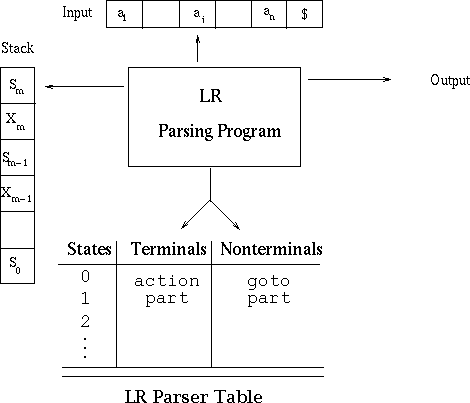
\includegraphics[height=0.7\textheight]{imageLR.png}
\end{center}
Actions : $\Aaccept$, $\Ashift\state$, $\Areduce{p}$, $\Areject$
\end{frame}

\begin{frame}{Soundness: dynamic checks \& safety}
  \begin{itemize}
  \item We have inserted dynamic checks in the interpreter
    \begin{itemize}
    \item Example: before reducing $E \rightarrow E\texttt{ + }E$, we check
      that the stack contains cells labelled $E$, \texttt{ + }, $E$
    \item Ensures type safety
    \item Also ensures soundness
    \end{itemize}
  \item New possible parsing outcome: $\Err$ (failure of the automaton)
  \item New question: may the tests fail ?
    \begin{itemize}
    \item Safety theorem
    \item Needs a safety validator
    \end{itemize}
  \end{itemize}
\end{frame}

% + 12min

\begin{frame}{Soundness theorem}
\begin{theorem}[Soundness]
\label{th:sound}
If $\parse{\stream}{n} = \Rparsed\sv{\stream'}$ holds, then there exists a
word $\word$ such that $\stream = \word \stream'$ and $\hsv{S}{\word}{\sv}$.
\end{theorem}
\begin{itemize}
\item Proof idea: the stack is a reduced form of the consumed input.
\end{itemize}
\end{frame}

\begin{frame}{Safety theorem}
\begin{theorem}[Safety]
\label{th:safety}
If the safety validator says ``yes'', then for every
input stream $\stream$ and for every integer ``fuel''~$n$,
$\parse{\stream}{n} \neq \Err$.
\end{theorem}
\begin{itemize}
\item The dynamic checks ensure that the stack has the expected
  shape.
\item Certificate for safety: abstract shape of the top of the stack for any given state.
\item Validator:
\begin{itemize}
\item ensures this invariant is preserved
\item ensures this invariant allows $\Areduce{p}$ and $\Aaccept$ actions
\end{itemize}
\end{itemize}
\end{frame}

% + 16 min

\begin{frame}{Completeness theorem}
\begin{theorem}[Completeness]
\label{th:complete}
If:
\begin{itemize}
\item the completeness validator says ``yes'' and
\item $\hsv{S}\word\sv$ holds,
\end{itemize}
then there exists $n_0$ such that for all $n\geq n_0$ and for all~$\stream$, either 
\begin{itemize}
\item $\parse{\word\stream}{n} = \Err$ or
\item $\parse{\word\stream}{n} = \Rparsed\sv\stream$.
\end{itemize}
\end{theorem}
\end{frame}

\begin{frame}{Completeness validation \& proof idea}
\begin{itemize}
\item Certificate for completeness: \lrone ``item sets''
\item Validation checks:
\begin{itemize}
\item closure properties of item sets
\item actions predicted by item sets are always present
\end{itemize}
\end{itemize}
\end{frame}

\begin{frame}{Conclusions}
\begin{itemize}
\item Framework for building provably correct \lrone parsers.
  \begin{itemize}
  \item light Coq proofs ($\sim 2500$ LOC)
  \end{itemize}
\item Possible improvements:
  \begin{itemize}
  \item termination in general case
  \item better performance
  \end{itemize}
\item Further work
  \begin{itemize}
  \item proving the lexer correct
  \item supporting precedence annotations on the grammar
  \end{itemize}
\end{itemize}
\end{frame}

% backup : lexer hack
% backup : d'autres énoncés

\end{document}
